\section{The User Interface (UI)}
\label{sec:ui}

While the Multi-Agent System can run autonomously, actual gameplay requires a ``Human-in-the-Loop'' (HITL) interface. The GUI was built natively in Java for seamless integration with Jason.
Since this front-end was outside the scope of the project, only the high-level design was hand-crafted, while \textbf{the code was primarily vibe-coded using Gemini Pro 3.1 and Claude Opus 4.6}.

\subsection{``Human'' Reasoner}
\label{subsec:human-player}

Implementing the interface to allow for human interaction bypasses the cognitive pipeline defined previously. Unlike autonomous agents, the human player does not utilize the \texttt{vesna.ProAgent} engine nor the epistemic trait matrix, relying entirely on their own heuristics.

For this reason, the Jason file (\texttt{reasoners/human/interface.asl}) simply defines a synchronization layer between the asynchronous GUI and the Jason execution cycle.

When the Narrator requests an action, the agent updates the GUI and then suspends its active intention, remaining idle until the user interacts with the interface. As demonstrated in Listing \ref{lst:human_vote_hook}, this physical interaction triggers a Java callback that injects the awaited belief directly into the agent's belief base. This new belief satisfies the blocking condition, restoring the plan and submitting the human's choice back to the Narrator.

\begin{lstlisting}[frame=single, language=Prolog, caption={Example of a UI execution hook. Once notified the start of the hunting phase the ui is updated to allow the voting; the Agent's intention to choose a target halts using \texttt{.wait} and resumes immediately once the human interaction injects the \texttt{user\_input} belief.}, label={lst:human_vote_hook}]
+!manage_phase(peasant_vote, Phase_title, Msg) 
    <-  ui.actions.start_vote(Phase_title, Msg, "vote");

+!choose_vote
    <-  .wait(user_input(RawTarget)); 
        -user_input(RawTarget); 
        .term2string(Target, RawTarget);
        !submit_vote(Target).
\end{lstlisting}

\subsection{Dashboard Layout and Visualizer}
\label{subsec:ui-layout}

To provide real-time transparency into the simulation, each player can instantiate\footnote{Each player can activate its own interface by adding \texttt{setting(spectator\_mode(true))} to their belief base. Furthermore, defining it inside the Narrator's belief base instantiates a windows for each player in the game} a dedicated graphical dashboard that acts as an explicit visualizer of its current state. As shown in Figure \ref{fig:ui_dashboard}, the interface is structurally divided into three panels:

\begin{figure}[H]
    \centering
    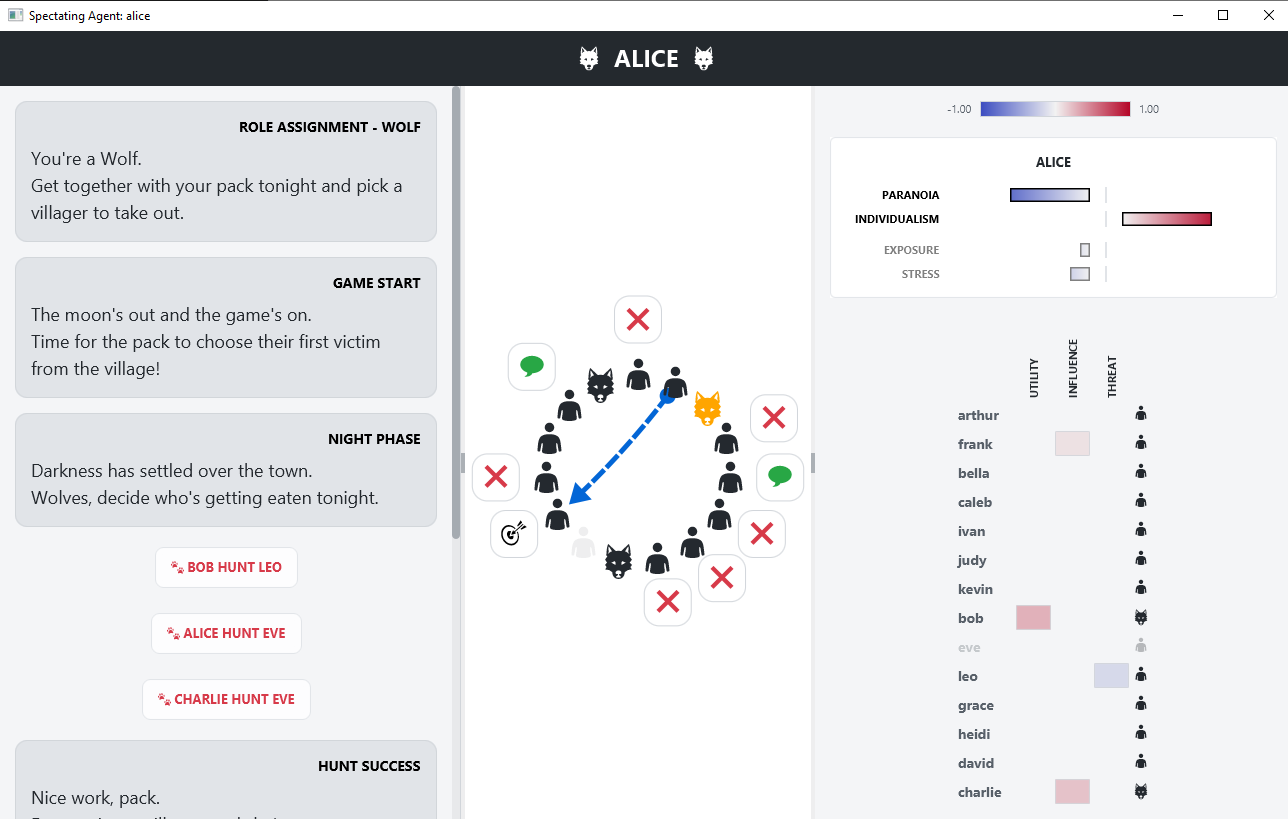
\includegraphics[width=1\textwidth]{images/UI.PNG}
    \caption{The real-time player dashboard. The left panel tracks the event log, the center maps directed actions, and the right exposes the agent's internal cognitive models. If interactions are needed, a fourth panel, centered on the bottom, appears and dictates what to do.}
    \label{fig:ui_dashboard}
\end{figure}

\begin{itemize}
    \item \textbf{Left Panel (Event Log):} Displays the chronological event sequence, encompassing Narrator announcements, broadcast messages from other agents, and a categorical recap of phase actions (e.g., hunting or voting summaries).
    \item \textbf{Center Panel (Spatial Graph):} Shows a circular node representation of all active players. It visually maps directed actions using arrows, explicitly tracing execution targets and the performatives of speech acts between agents.
    \item \textbf{Right Panel (Cognitive State):} Visualizes the agent's internal \textbf{world model}, tracking both its affective \texttt{temper} (mood and personality parameters) and its epistemic belief matrix regarding other players in real time\footnote{By design, this panel is completely disabled if the dashboard is assigned to a human player, as they do not need the engine's internal trait modeling or affective heuristics.}.
\end{itemize}

For human-driven players, the dashboard is mandatory, and transitions from a passive visualizer to an active input mechanism. When the agent's execution hook pauses to await a decision (as detailed in Section \ref{subsec:human-player}), the UI explicitly prompts the human operator for action.